\documentclass[11pt,a4paper]{article}

\usepackage[margin=1in]{geometry}
\usepackage{graphicx}
\usepackage{booktabs}
\usepackage{amsmath}
\usepackage{siunitx}
\usepackage{caption}
\usepackage{subcaption}
\usepackage{float}
\usepackage[hidelinks]{hyperref}
\usepackage{enumitem}
\usepackage{xcolor}
\usepackage{titlesec}

\graphicspath{{../figures/}}
\captionsetup{font=small,labelfont=bf}
\titleformat{\section}{\normalfont\Large\bfseries}{\thesection}{0.6em}{}
\titleformat{\subsection}{\normalfont\large\bfseries}{\thesubsection}{0.6em}{}
\setlist{itemsep=2pt,topsep=3pt}

\newcommand{\best}[1]{\textbf{#1}}

\title{\vspace{-1.2cm}\textbf{The Effect of Content Embeddings on Hybrid\\ Recommender Systems for Short Videos}\\[0.3em]
\large A study on the VK-LSVD dataset}
\author{}
\date{July 2026}

\begin{document}
\maketitle
\vspace{-1.0cm}

\begin{abstract}
\noindent
Hybrid recommenders combine collaborative filtering with content features, but it is
often unclear when the content side actually pays off. This report measures that on
VK-LSVD, an industrial short-video dataset with a single multimodal content embedding
per item whose components are ordered, so a prefix of length $d$ is a usable
lower-dimensional signal. I train and compare six model families, from a popularity
baseline to a two-tower network, and evaluate them under a global temporal split with
cold, warm, and popular item slices. The result is consistent across three ways of
adding the embedding: content signal barely moves quality on popular items and carries
almost all of its value on cold items with little training history. Any pure
collaborative model scores exactly zero on the cold slice; a hybrid that reserves a
fixed quota of content-selected candidates lifts cold NDCG@10 from $0$ to $0.0023$ on
the test week while keeping overall metrics on par with iALS. Quality as a function of
$d$ saturates past $d=32$, and the multimodal embedding contributes far more than
tabular metadata ($+22\%$ vs.\ $+2\%$ NDCG@10 in the two-tower model).
\end{abstract}

\section{Introduction}
Recommender systems for short-video feeds have to rank a catalog that changes by the
hour. Collaborative filtering (CF) learns from interaction history and does this well
for items people have already watched, but it has nothing to say about a video uploaded
an hour ago. Content features are the usual answer: if two videos look and sound
similar, a model can transfer preference from one to the other before either has much
history. The open question this report addresses is narrower and more practical than
``do content features help.'' It is \emph{when} they help, and by how much, relative to
the cost of adding them.

VK-LSVD~\cite{vklsvd} gives an unusually clean setting for that question. It ships one
multimodal content embedding per video, trained only on content (frame, description,
audio) with no collaborative signal mixed in. The embedding has a property most datasets
lack: its 64 components are ordered so that the dot product of the first $n$ components
approximates the cosine similarity of the full production embedding. That turns
``how much content signal do you need'' into a single knob, the prefix length $d$, and
lets me trace a clean quality-versus-width curve instead of guessing at a fixed size.

\section{Problem Statement}
The task defined for this project is to implement several collaborative filtering
algorithms on an open dataset, add content embeddings of different kinds, and report how
each addition changes recommendation accuracy, robustness, and ranking quality. VK-LSVD
provides a single multimodal embedding rather than separate text, image, and audio
vectors, so the ``different kinds of embedding'' axis is reframed. Instead of comparing
modalities, I study how informative the multimodal signal is as a function of two things
I can control: its width (the prefix length $d$) and the way it enters the model (a pure
content model, a fallback hybrid, or a learned feature inside a neural retriever). The
central claim I set out to test is that content embeddings pay off mainly on cold items
and add little on popular ones. That claim, if it holds, is the direct answer to the
``in different scenarios'' part of the task.

\section{Objectives}
\begin{enumerate}[label=\textbf{O\arabic*.},leftmargin=2.4em]
  \item Build a reproducible pipeline over a VK-LSVD subsample: interaction loading, an
        implicit-feedback target, a global temporal split, and ranking metrics with
        cold/warm/popular slices.
  \item Implement and compare six model families spanning the CF-to-hybrid spectrum:
        Popularity, content k-NN, iALS, BPR, EASE, and a two-tower network.
  \item Trace quality against embedding width $d\in\{4,8,16,32,64\}$ for every model
        that consumes the embedding.
  \item Separate the contribution of the content embedding from that of tabular
        metadata (duration, demographics).
  \item Confirm the findings transfer to a second, much denser subsample and to the
        held-out test week.
\end{enumerate}

\noindent I frame three hypotheses and test each in Section~\ref{sec:results}:
\begin{itemize}
  \item[\textbf{H1.}] Content signal drives the gain on cold items and barely affects
        popular ones.
  \item[\textbf{H2.}] Quality rises with $d$ and then saturates; the first components
        hold most of the information.
  \item[\textbf{H3.}] Tabular metadata alone contributes much less than the content
        embedding.
\end{itemize}

\section{Dataset and Exploratory Analysis}
VK-LSVD is the largest open industrial short-video dataset: 40 billion interactions,
10 million users, 20 million videos, over six consecutive months. I work on the official
\texttt{ur0.01\_ir0.01} subsample (a random 1\% of users by 1\% of items):
3.72M interactions, 89{,}371 users, 120{,}415 videos. To check that the conclusions are
not an artifact of one sampling regime, I also use the dense \texttt{up0.001\_ip0.001}
subsample (10{,}000 users, 19{,}628 videos, 47M interactions, 24\% density against
0.036\% for the main one).

Each interaction records watch time, explicit reactions (like, dislike, share, bookmark,
click-on-author, open-comments) and context. There are no repeated exposures of the same
pair. Item metadata gives duration and author; user metadata gives age, gender, and
region.

\begin{figure}[H]
  \centering
  \begin{subfigure}{0.48\textwidth}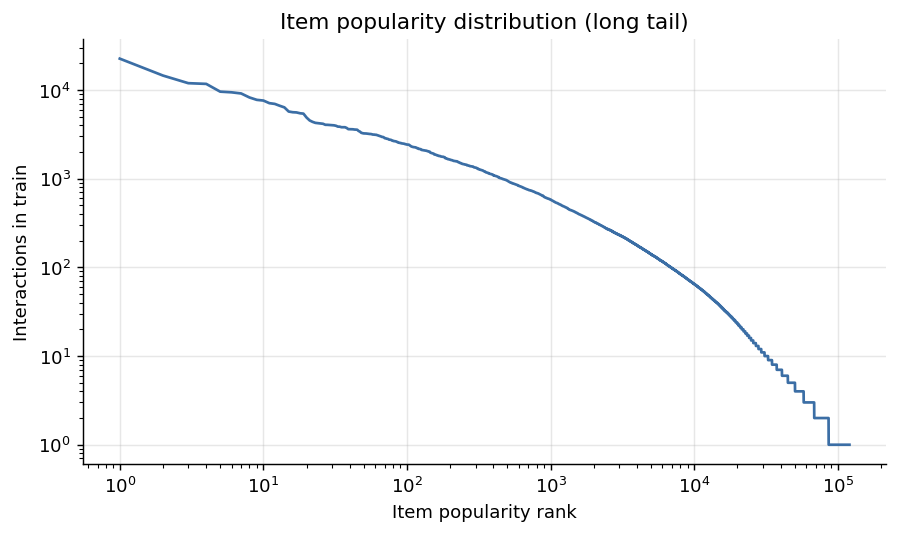
\includegraphics[width=\linewidth]{01_item_longtail.png}\caption{Item popularity (log-log).}\end{subfigure}\hfill
  \begin{subfigure}{0.48\textwidth}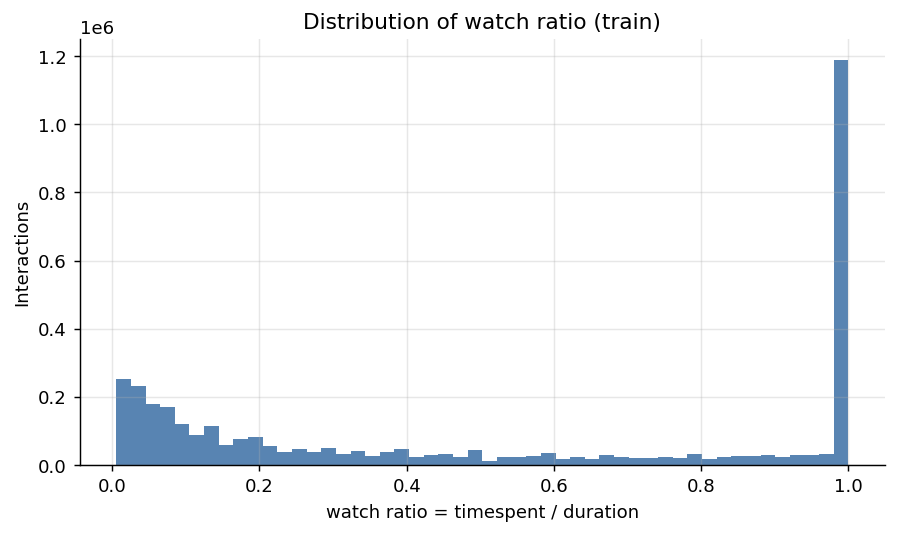
\includegraphics[width=\linewidth]{02_watch_ratio.png}\caption{Watch ratio.}\end{subfigure}
  \\[0.5em]
  \begin{subfigure}{0.48\textwidth}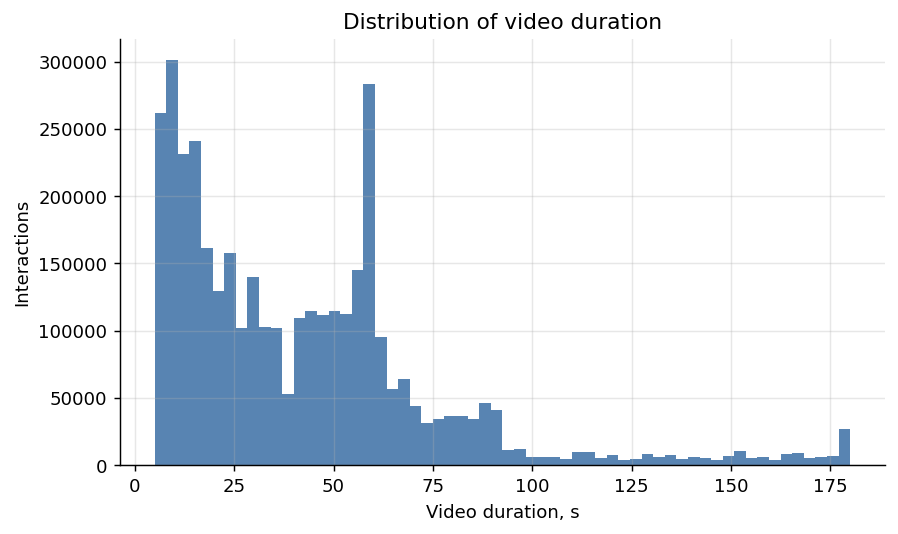
\includegraphics[width=\linewidth]{03_duration.png}\caption{Video duration.}\end{subfigure}\hfill
  \begin{subfigure}{0.48\textwidth}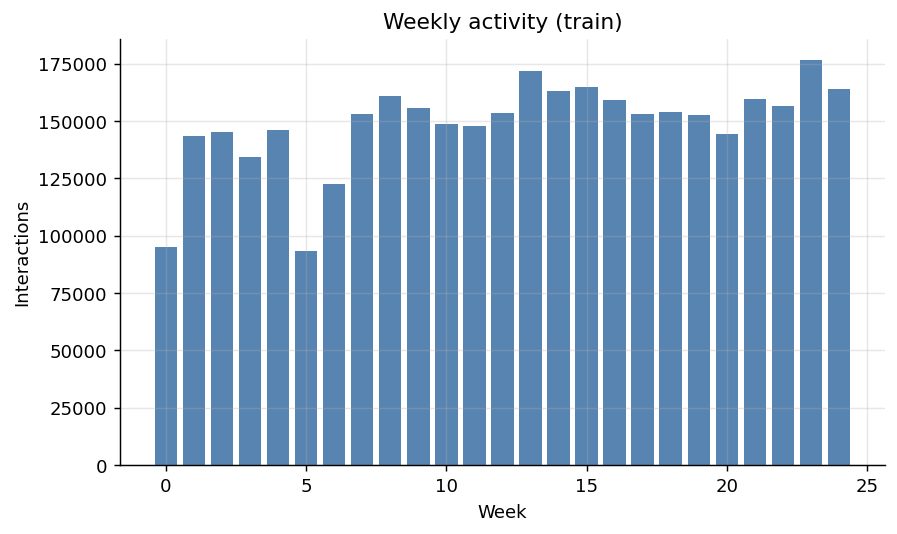
\includegraphics[width=\linewidth]{04_weekly_activity.png}\caption{Weekly activity.}\end{subfigure}
  \caption{Exploratory views of the main subsample (train weeks 0--24).}
  \label{fig:eda}
\end{figure}

Two properties of the data shaped the design. Explicit reactions cover only 3.4\% of
interactions, so a target built on likes alone would be extremely sparse. And 31\% of
views have \texttt{timespent} $\geq$ \texttt{duration}: these are looped replays, a
short-video quirk, for which the watch ratio is clipped to 1.

\section{Methodology}
\subsection{Implicit-feedback target}
A positive interaction is defined as \texttt{like OR share OR bookmark OR}
watch-ratio $\geq 0.8$ (the \emph{combined} target). Two alternatives are tested in
Section~\ref{sec:target}: explicit reactions only, and watch-ratio $\geq 0.5$. The watch
ratio is \texttt{timespent}/\texttt{duration}, clipped to $[0,1]$.

\subsection{Global temporal split}
I use the split shipped with the dataset: train is weeks 0--24, validation is week 25,
test is week 26. The model learns from the past and is scored on the future. Random and
leave-one-out splits are avoided because they leak future information and inflate
metrics. Users and items that first appear in the evaluation weeks are kept, not dropped;
they form the cold slices. Hyperparameters were tuned on validation only. The test week
was touched once, with the final models.

\subsection{Models}
\begin{itemize}
  \item \textbf{Popularity} --- top-$N$ by number of train positives; the lower bound.
  \item \textbf{Content k-NN} --- a pure content model. The user profile is the mean of
        the embeddings of their train positives; items are scored by cosine similarity.
  \item \textbf{iALS}~\cite{hu2008} --- CF with confidence weighting
        $1 + \alpha(\text{watch\_ratio} + 3\cdot\text{like})$, $\alpha=20$, 128 factors.
  \item \textbf{BPR-MF}~\cite{rendle2009} --- matrix factorization with a pairwise
        ranking loss.
  \item \textbf{EASE}~\cite{steck2019} --- a closed-form linear item-item model. The
        dense item-by-item matrix needs about 62~GB on the full catalog, so EASE is
        trained on the dense subsample (19{,}628 items, $\approx$1.5~GB) instead.
  \item \textbf{iALS + content fallback} --- a hybrid. Warm items are ranked by iALS;
        cold candidates are selected by content similarity to the user profile and given
        a fixed 10\% quota of output positions (the exploration-slot pattern used in
        production feeds).
  \item \textbf{Two-tower}~\cite{covington2016} --- a neural retriever. The item tower is
        \texttt{concat(id\_emb, frozen content\_emb $\to$ learned projection,
        duration\_bucket)} $\to$ MLP; the user tower is \texttt{id\_emb + demographics}
        $\to$ MLP. Training uses InfoNCE~\cite{oord2018} with in-batch negatives plus
        popularity-sampled hard negatives, L2-normalized outputs, temperature 0.07.
\end{itemize}

\subsection{Evaluation protocol}
Ranking is done over the full catalog, without sampled negatives. Accuracy metrics are
Recall@10/50, NDCG@10/50, and MAP@10. Beyond-accuracy metrics are catalog Coverage@50
and Novelty@10 (the mean $-\log_2$ popularity share of recommended items). Robustness
slices split evaluation items into cold ($<5$ train interactions), warm, and popular
(top 1\%), and split users into cold (no train history, served the popularity fallback)
and active. Evaluation runs in the original id space: items with no train history are
legitimately unreachable for a pure CF model, and that is exactly the effect being
measured.

\section{Experiments and Results}
\label{sec:results}
\subsection{Model comparison}
\begin{table}[H]
\centering
\small
\caption{Model comparison on validation (week 25). R = Recall, N = NDCG; cold/warm are NDCG@10 on item slices. Best per column in bold.}
\label{tab:val}
\begin{tabular}{lrrrrrrrr}
\toprule
Model & R@10 & N@10 & R@50 & N@50 & N@10$_{\text{cold}}$ & N@10$_{\text{warm}}$ & Cov@50 & Nov@10 \\
\midrule
Popularity              & 0.0002 & 0.0001 & 0.0127 & 0.0030 & 0.0000 & 0.0000 & 0.001 & 8.7 \\
Content k-NN ($d{=}64$) & 0.0028 & 0.0017 & 0.0111 & 0.0038 & 0.0016 & 0.0017 & 0.614 & 18.0 \\
BPR-MF                  & 0.0212 & 0.0123 & 0.0676 & 0.0242 & 0.0000 & \best{0.0179} & 0.488 & 14.7 \\
iALS                    & \best{0.0312} & \best{0.0170} & \best{0.1107} & \best{0.0373} & 0.0000 & 0.0084 & 0.098 & 11.2 \\
iALS + fallback         & 0.0299 & 0.0164 & 0.1097 & 0.0369 & \best{0.0036} & 0.0074 & 0.114 & 12.1 \\
Two-tower: id-only      & 0.0051 & 0.0029 & 0.0248 & 0.0078 & 0.0004 & 0.0047 & 0.991 & 18.4 \\
Two-tower: + metadata   & 0.0054 & 0.0029 & 0.0250 & 0.0078 & 0.0005 & 0.0047 & \best{0.993} & 18.5 \\
Two-tower: + embedding  & 0.0060 & 0.0032 & 0.0270 & 0.0085 & 0.0010 & 0.0049 & 0.992 & \best{18.6} \\
Two-tower: full hybrid  & 0.0067 & 0.0035 & 0.0291 & 0.0090 & 0.0015 & 0.0050 & \best{0.993} & 18.4 \\
\bottomrule
\end{tabular}
\end{table}

\begin{figure}[H]
  \centering
  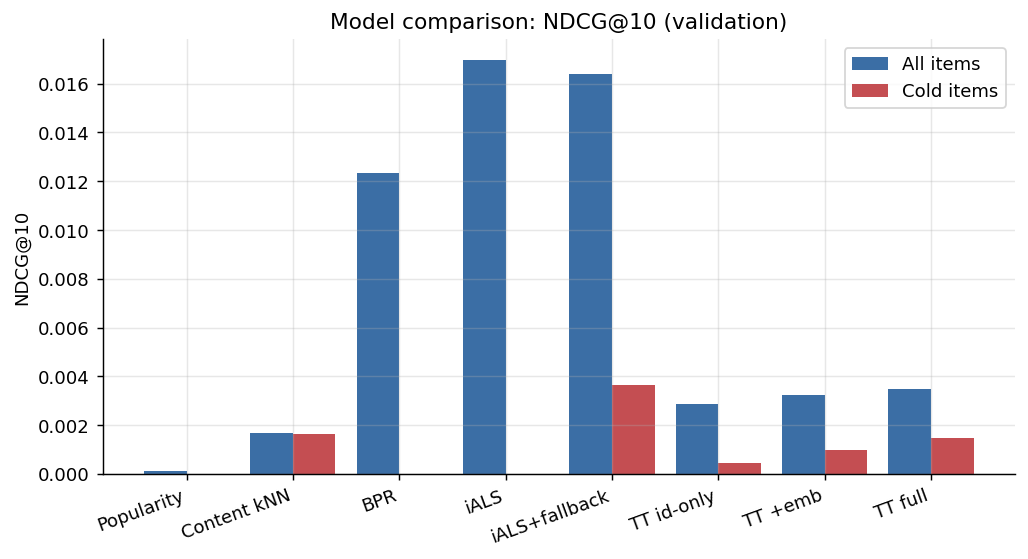
\includegraphics[width=0.78\textwidth]{08_model_comparison.png}
  \caption{Overall and cold-slice NDCG@10 on validation. Every pure CF model scores zero on the cold slice.}
  \label{fig:modelcmp}
\end{figure}

Table~\ref{tab:val} and Figure~\ref{fig:modelcmp} tell one story. Pure CF (iALS,
NDCG@10 $=0.0170$) wins the overall ranking by a wide margin, but on cold items it scores
exactly zero, because those items are absent from the training matrix. The content k-NN
model is an order of magnitude weaker overall, yet it is the only baseline that reaches
cold items at all (cold NDCG@10 $=0.0016$). The fallback hybrid gets both: its cold
NDCG@10 of $0.0036$ is the best of any model, and it costs only a 3\% drop in overall
quality against iALS. This is the first evidence for H1.

\subsection{Width of the content signal}
\begin{table}[H]
\centering
\small
\caption{NDCG@10 as a function of embedding width $d$ (validation), for three ways of using the embedding.}
\label{tab:dablation}
\begin{tabular}{lrrrrrr}
\toprule
 & \multicolumn{2}{c}{Content k-NN} & \multicolumn{2}{c}{iALS + fallback} & \multicolumn{2}{c}{Two-tower} \\
\cmidrule(lr){2-3}\cmidrule(lr){4-5}\cmidrule(lr){6-7}
$d$ & overall & cold & overall & cold & overall & cold \\
\midrule
4  & 0.0001 & 0.0001 & 0.0154 & 0.0008 & 0.0024 & 0.0004 \\
8  & 0.0006 & 0.0010 & 0.0157 & 0.0018 & 0.0028 & 0.0007 \\
16 & 0.0010 & 0.0009 & 0.0160 & 0.0022 & 0.0034 & 0.0012 \\
32 & 0.0016 & 0.0017 & 0.0164 & \best{0.0036} & 0.0035 & 0.0012 \\
64 & 0.0017 & 0.0016 & 0.0164 & \best{0.0036} & 0.0032 & 0.0010 \\
\bottomrule
\end{tabular}
\end{table}

\begin{figure}[H]
  \centering
  \begin{subfigure}{0.48\textwidth}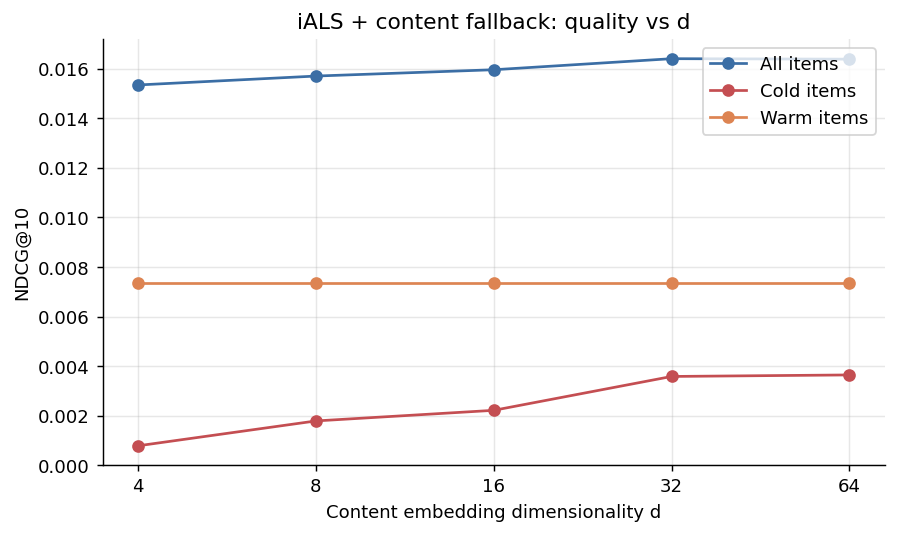
\includegraphics[width=\linewidth]{06_hybrid_ndcg_vs_d.png}\caption{iALS + fallback.}\end{subfigure}\hfill
  \begin{subfigure}{0.48\textwidth}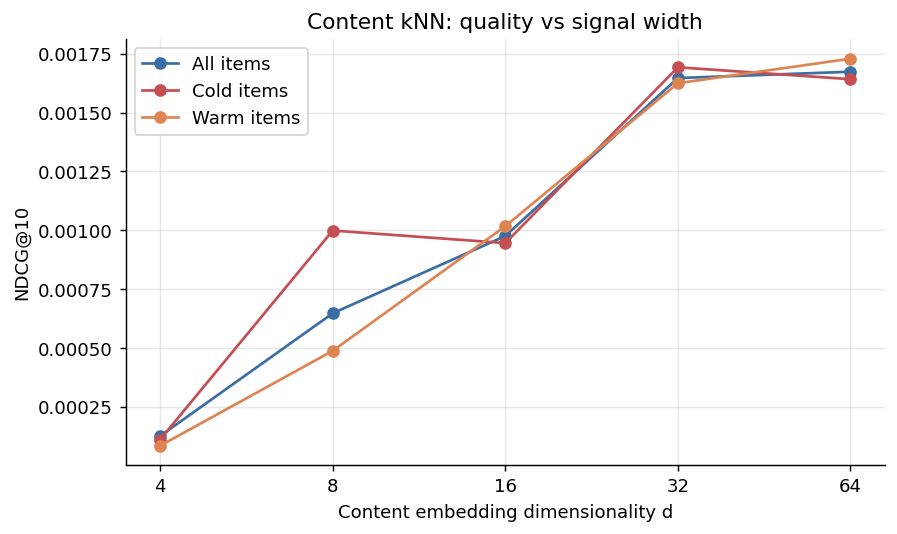
\includegraphics[width=\linewidth]{05_knn_ndcg_vs_d.png}\caption{Content k-NN.}\end{subfigure}
  \\[0.5em]
  \begin{subfigure}{0.48\textwidth}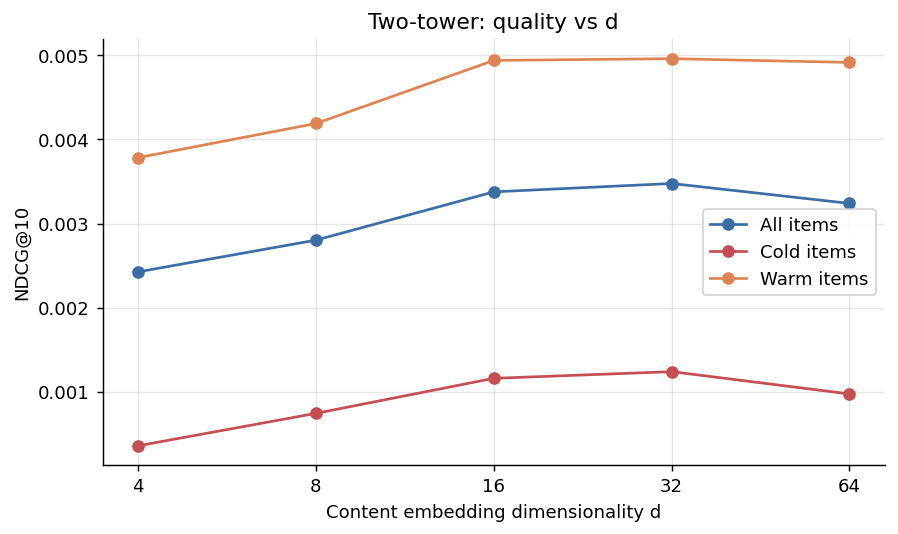
\includegraphics[width=\linewidth]{07_tt_ndcg_vs_d.png}\caption{Two-tower.}\end{subfigure}
  \caption{Quality against embedding width $d$. The warm line is flat; the cold line climbs and then levels off past $d=32$.}
  \label{fig:dcurve}
\end{figure}

The three integration methods trace the same shape (Table~\ref{tab:dablation},
Figure~\ref{fig:dcurve}): a fast climb up to $d=16$--$32$, then a plateau at $d=64$. For
the hybrid, cold NDCG@10 rises from $0.0008$ at $d=4$ to $0.0036$ at $d=32$ and stops
moving after that. The first components carry most of the information, which confirms H2
and has a direct practical reading: $d=32$ is enough in production, halving the memory
and compute of the content path for no measurable loss.

\subsection{Embedding vs.\ metadata}
Under a fixed training budget (8 epochs, CPU), adding the content embedding raises the
two-tower NDCG@10 by 22\% over id-only ($0.0035$ vs.\ $0.0029$), while tabular metadata
alone adds 2\% ($0.0029$, statistically flat). On the cold slice the full hybrid reaches
$3.4\times$ the id-only model. That is H3: the multimodal embedding is the content signal
that matters, and metadata is a weak add-on.

\subsection{Target ablation}
\label{sec:target}
\begin{table}[H]
\centering
\small
\caption{iALS metrics under three positive-interaction definitions (validation).}
\label{tab:target}
\begin{tabular}{lrrrrr}
\toprule
Positive definition & Positives share & R@10 & N@10 & R@50 & N@50 \\
\midrule
explicit (like/share/bookmark) & 3.4\%  & 0.0289 & 0.0147 & 0.0795 & 0.0268 \\
watch (ratio $\geq 0.5$)       & 48.8\% & 0.0311 & \best{0.0172} & \best{0.1114} & \best{0.0383} \\
combined (main)                & 39.8\% & \best{0.0312} & 0.0170 & 0.1107 & 0.0373 \\
\bottomrule
\end{tabular}
\end{table}

A target built only on explicit reactions loses 28\% of Recall@50 against the combined
target: the implicit watch signal is needed. The gap between watch and combined is small,
but combined also captures explicit intent, so I keep it as the fuller definition.

\subsection{Beyond accuracy}
Content sharply widens catalog coverage. Coverage@50 is 9.8\% for iALS, 11.4\% for the
hybrid, 61\% for content k-NN, and 99\% for the two-tower with the embedding. Novelty
rises monotonically as content is added (11.2 for iALS, 12.1 for the hybrid, 18.6 for the
two-tower). Content is a lever against the popularity feedback loop, a separate benefit
from accuracy.

\subsection{Final evaluation on test}
\begin{table}[H]
\centering
\small
\caption{Final evaluation on test (week 26). Stochastic models report mean $\pm$ std over 3 seeds.}
\label{tab:test}
\begin{tabular}{lrrrr}
\toprule
Model & R@10 & N@10 & R@50 & N@10$_{\text{cold}}$ \\
\midrule
Popularity              & 0.0000 & 0.0000 & 0.0115 & 0.0000 \\
Content k-NN ($d{=}64$) & 0.0022 & 0.0013 & 0.0087 & 0.0010 \\
EASE (dense subsample)  & 0.0011 & 0.0009 & 0.0067 & 0.0000 \\
BPR-MF                  & $0.0164 \pm 0.0004$ & $0.0092 \pm 0.0002$ & $0.0539 \pm 0.0004$ & $0.0000$ \\
iALS                    & $\mathbf{0.0218 \pm 0.0002}$ & $\mathbf{0.0118 \pm 0.0000}$ & $0.0840 \pm 0.0001$ & $0.0000$ \\
iALS + fallback         & $0.0213 \pm 0.0003$ & $0.0116 \pm 0.0001$ & $\mathbf{0.0849 \pm 0.0006}$ & $\mathbf{0.0023 \pm 0.0000}$ \\
\bottomrule
\end{tabular}
\end{table}

The validation ordering holds on the test week (Table~\ref{tab:test}). iALS is still the
strongest overall; the hybrid keeps parity on the general metrics (its Recall@50 is
actually higher) and is the only model with a non-zero cold slice. Seed variance is
negligible ($\sigma \leq 0.0004$). EASE on the dense subsample trails iALS: in a
very high density regime, a linear item-item model is not enough.

\section{Conclusions}
\begin{itemize}
  \item \textbf{H1 holds.} Content embeddings barely change quality on popular items, but
        they move the cold slice from a hard zero (every pure CF model) to measurable
        quality. The best mechanism is the hybrid with a content candidate quota:
        cold NDCG@10 $=0.0036$ at a 3\% overall cost.
  \item \textbf{H2 holds.} The quality-versus-$d$ curve saturates past $d=32$ in all three
        integration methods; half of the embedding is enough.
  \item \textbf{H3 holds.} Metadata adds 2\% against 22\% for the embedding (two-tower,
        NDCG@10); the multimodal embedding is the content signal that counts.
  \item \textbf{Practical reading.} When the catalog is stable and items live long, plain
        iALS is enough. When the catalog turns over fast, which is the short-video case, a
        content fallback is not optional: without it, new items are systematically never
        recommended. The cold-candidate quota is a transparent dial on the
        accuracy-versus-exploration trade-off.
  \item Content also improves coverage and novelty in every configuration, a benefit
        beyond top-$k$ accuracy.
\end{itemize}

\section{Limitations}
\begin{itemize}
  \item One multimodal embedding rather than separate text, image, and audio vectors, so
        the modality comparison is replaced by the width axis $d$.
  \item Subsamples rather than the full 452~GB dataset. Transfer was checked on a second
        subsample with very different density.
  \item The two-tower model was trained under a small CPU budget (8 epochs) and does not
        reach iALS in absolute terms; its relative effects (embedding contribution, shape
        of the $d$ curve) agree with the other models. LightFM was dropped because it does
        not build under Python 3.12.
  \item The two-tower test-week run was not completed for compute reasons; its numbers are
        reported on validation.
  \item Offline metrics are not the same as online effect; the cold-slice finding should
        be confirmed with an A/B test.
\end{itemize}

\begin{thebibliography}{9}
\bibitem{vklsvd} deepvk. \emph{VK-LSVD: Large Short-Video Dataset}. 2026.
  \url{https://huggingface.co/datasets/deepvk/VK-LSVD} (accepted at WWW~'26).
\bibitem{hu2008} Y.~Hu, Y.~Koren, C.~Volinsky. Collaborative Filtering for Implicit
  Feedback Datasets. \emph{ICDM}, 2008.
\bibitem{rendle2009} S.~Rendle et al. BPR: Bayesian Personalized Ranking from Implicit
  Feedback. \emph{UAI}, 2009.
\bibitem{steck2019} H.~Steck. Embarrassingly Shallow Autoencoders for Sparse Data.
  \emph{WWW}, 2019.
\bibitem{covington2016} P.~Covington, J.~Adams, E.~Sargin. Deep Neural Networks for
  YouTube Recommendations. \emph{RecSys}, 2016.
\bibitem{oord2018} A.~van~den~Oord, Y.~Li, O.~Vinyals. Representation Learning with
  Contrastive Predictive Coding. \emph{arXiv:1807.03748}, 2018.
\end{thebibliography}

\end{document}
